\documentclass{beamer}
\usepackage{beamerthemesplit} % 加载主题宏包
%\usetheme{Warsaw} % 选用该主题
%\usetheme{Dresden}
\usetheme{Boadilla}
%\usetheme{CambridgeUS}
\usecolortheme{dolphin}

\usefonttheme{serif}
%\usecolortheme{rose}
\usepackage{multirow}
\usepackage{subfig}
\usepackage{amssymb,amsmath,mathtools}
\usepackage{amsfonts,booktabs}
\usepackage{lmodern,textcomp}
\usepackage{color}
\usepackage{tikz}
\usepackage{natbib}
\usepackage{multicol}
\usepackage{graphicx} % Required for inserting images
\usepackage{ctex}
\usepackage{hyperref}
\usepackage{nicefrac}
\usepackage{tabularx}
\usepackage{ragged2e}
\usepackage{booktabs}
\setbeamertemplate{caption}[numbered]

\title[Trade and Innovation]{Trade and Innovation}
\author{陈宠\inst{1}}
\institute{
    中国人民大学经济学院\inst{1}
    }

\date{2026年5月7日}

\begin{document}
\maketitle
%目录
\begin{frame}
    \tableofcontents
\end{frame}

% Part I
\section{创新\(\Longrightarrow\)贸易}
\begin{frame}
\begin{center}
    \begin{minipage}{1\textwidth}
	\setbeamercolor{mybox}{fg=white, bg=black!50!blue}
		\begin{beamercolorbox}[wd=0.70\textwidth, rounded=true, shadow=true]{mybox}
			\LARGE \centering 创新\(\Longrightarrow\)贸易
		\end{beamercolorbox}
    \end{minipage}
\end{center} 
\end{frame}

\subsection{引力方程(Gravity Equation)}
\begin{frame}{一个实证证据：Gravity Equation}
\begin{itemize}
    \item 万有引力模型：
\[F=G\frac{m_1\times m_2}{r^2}\]
    \item 贸易引力模型：
    \[X_{ij}=\alpha\frac{Y_i\times Y_j}{d_{ij}}\]
\(X_{ij}\)：贸易流；\(Y\)：GDP；\(d\)：距离
\end{itemize}
\begin{figure}
    \centering
    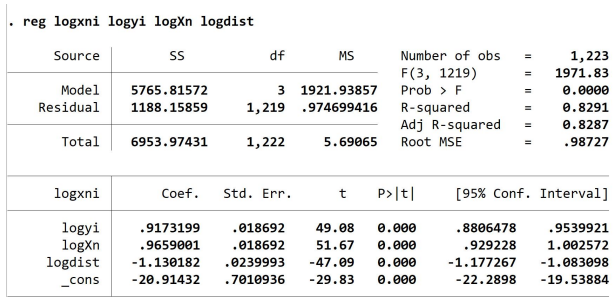
\includegraphics[width=0.7\linewidth]{Gravity Equation.png}
    \caption{贸易引力模型回归}
\end{figure}
\end{frame}

\subsection{阿明顿模型（Armington Model）}
\begin{frame}{Armington Model}
\begin{itemize}
    \item 假设：
    \begin{itemize}
        \item CES Preference(Love-of-Variety)
        \item 单一劳动生产要素
        \item 完全竞争市场
    \end{itemize}
\[U_{j}=\left(\sum_{i\in S}a_{ij}^{\frac{1}{\sigma}}q_{ij}^{\frac{\sigma-1}{\sigma}}\right)^{\frac{\sigma}{\sigma-1}}\]
\[\sum_{i\in S}p_{ij}q_{ij}\leq Y_{j}\]
\[\Longrightarrow q_{ij}=a_{ij}p_{ij}^{-\sigma}Y_{j}P_{j}^{\sigma-1}\]
\[\Longrightarrow X_{ij}=p_{ij}q_{ij}=a_{ij}\tau_{ij}^{1-\sigma}\left(\frac{w_{i}}{A_{i}}\right)^{1-\sigma}P_{j}^{\sigma-1}Y_{j}\]
\[\Longrightarrow U_j=\lambda_{jj}^\frac{1}{1-\sigma}A_j\]
\end{itemize}
\end{frame}


\subsection{比较优势（Comparative Advantage）}
\begin{frame}{一个典型理论：Ricardo Comparative Advantage}
\begin{itemize}
    \item 假设：
    \begin{itemize}
        \item 两国\(\times\)两商品
        \item 自由贸易、无运输成本、劳动力不能跨国流动
        \item 平均生产成本固定
    \end{itemize}
\end{itemize}
\begin{table}[htbp]
  \centering
  \caption{李嘉图的例子}
  \begin{tabular}{lcc}
    \hline
     & Britain & Portugal \\
    \hline
    \quad Labor Demand of Wine & 120 & 80 \\
    \quad Labor Demand of Cloth & 100 & 90 \\
    \hline
    \# of Workers & 1200 & 1200 \\
    \hline
  \end{tabular}
\end{table}
\begin{itemize}
    \item 生产率差异：\(\frac{A_{B,Wine}}{A_{B,Cloth}}=0.833\),\(\frac{A_{P,Wine}}{A_{P,Cloth}}=1.125\)
    \item 经济学直觉：贸易由生产率的差异驱动
\end{itemize}
\end{frame}

\subsection{新贸易理论（E-K Model）}
\begin{frame}{新贸易理论（E-K Model）}
\begin{itemize}
    \item 假设：
    \begin{itemize}
        \item 边际产出成本\(c_i\)恒定
        \item 异质性企业的生产率服从Frechet分布，\(\Pr\{Z_{i}(\omega)\leq z\}=\exp\{-A_{i}z^{-\theta}\}\)
    \end{itemize}
\[p_{ij}(\omega)=\frac{\tau_{ij}c_i}{Z_i(\omega)}\]
\[\Longrightarrow\lambda_{ij}=\Pr\{p_{ij}(\omega)\leq\min_{k\in S,k\neq i}p_{kj}(\omega)\}=\frac{A_{i}\left(c_{i}\tau_{ij}\right)^{-\theta}}{\sum_{i'\in S}A_{i'}\left(c_{i'}\tau_{i'j}\right)^{-\theta}}\]
\[\Longrightarrow U_j=\frac{w_{i}}{P_{i}}=\lambda_{ii}^{-\frac{1}{\theta}}A_{i}^{\frac{1}{\theta}}\]
\end{itemize}
\end{frame}

\subsection{Frechet分布}
\begin{frame}{Frechet分布}
\begin{itemize}
    \item Frechet分布是否合理？
    \begin{itemize}
        \item 数据层面的合理性：肥尾分布——大公司总是少的
        \item Frechet分布有不错的微观基础
    \end{itemize}
\end{itemize}
\begin{itemize}
    \item 企业无时无刻都在想某种产品的创新，我们用\(Z\)来刻画产生创意的效率，我们假定这一效率服从Pareto Distribution：
\[F(z)=\Pr(Z\leq z)=1-\left(\frac{z}{\underline{z}}\right)^{-\theta},z\geq\underline{z}\]
\begin{itemize}
    \item 该分布由两个参数决定：\(\underline{z}\)表示创意质量下界、\(\theta\)描述了帕累托分布的形状
\end{itemize}
    \item \(N\)个创意中，效率高于\(z\)的创意的数量\(N_z\)服从二项分布
\[\Pr(N_{z}=n)=C_{N}^{n}\times p_{z}^{n}\left(1-p_{z}\right)^{N-n},p_z=1-F(z)\]
    \item 高质量创意\(N_z\)的期望值\(\mathbb{E}\left[N_z\right]\)
\[\mathbb{E}\left[N_z\right]=p_z\times N=N\underline{z}^{\theta}z^{-\theta}\]
\end{itemize}
\end{frame}

\begin{frame}{Frechet分布}
\begin{itemize}
    \item 从二项分布到泊松分布：
\end{itemize}
我们让出现创意的数量无限多\(N\rightarrow\infty\)，创意效率的下限无限的低\(\underline{z}\rightarrow 0\)，且他们改变的速度使得\(T=N\underline{z}^{\theta}\)、\(\lambda=E[N_{z}]=Tz^{-\theta}\)保持不变
\footnotesize
\begin{align*}
    \Pr(N_{z}=n)&=\frac{N!}{n!\left(N-n\right)!}\times p_{z}^{n}\left(1-p_{z}\right)^{N-n}\\&=\frac{\left(N-n+1\right)\times\cdots\times\left(N-1\right)\times N}{n!}\times p_{z}^{n}\left(1-p_{z}\right)^{N-n}\\&=\frac{\left(N-n+1\right)\times\cdots\times\left(N-1\right)\times N}{N^{n}}\frac{N^{n}}{n!}\left(\frac{\lambda}{N}\right)^{n}\left(1-\frac{\lambda}{N}\right)^{N-n}\\&=\frac{\left(N-n+1\right)\times\cdots\times\left(N-1\right)\times N}{N^{n}}\frac{\lambda^{n}}{n!}\left(1-\frac{\lambda}{N}\right)^{N}\left(1-\frac{\lambda}{N}\right)^{-n}
\end{align*}
\[\Longrightarrow \lim_{N\rightarrow\infty}\Pr(N_{z}=n)=\frac{\lambda^{n}}{n!}e^{-\lambda}\]
\end{frame}

\begin{frame}{Frechet分布}
    \begin{itemize}
        \item 从泊松分布到Frechet分布
    \end{itemize}
我们使用\(Z^{(k)}\)记录第\(k\)有效率的创意的效率，即\(Z^{(1)}>Z^{(2)}>Z^{(3)}>\cdots\)。那么第\(k\)有效率创意出现的概率，意味着前面最少有\(k-1\)个创意比它更有效率：
\begin{align*}
    \Pr[Z^{(k)}\leq z]&=\Pr[Z^{(1)}>z\cup Z^{(2)}>z\cup\cdots\cup Z^{(k-1)}>z]\\&=\sum_{l=1}^{k-1}\Pr(N_{z}=l)=e^{-\lambda}\sum_{l=1}^{k-1}\frac{\lambda^{l}}{l!}\\&=e^{-Tz^{-\theta}}\sum_{l=1}^{k-1}\frac{\left(Tz^{-\theta}\right)^{l}}{l!}
\end{align*}
当我们只考虑最有效率的创意\(k-1\)时，
\[\Pr[Z^{(1)}\leq z]=e^{-Tz^{-\theta}}\]
\begin{itemize}
    \item 这一分布我们称之为Frechet分布，或第二类极值分布
\end{itemize}
\end{frame}

%Part II
\section{贸易\(\Longrightarrow\)创新}
\begin{frame}
\begin{center}
    \begin{minipage}{1\textwidth}
	\setbeamercolor{mybox}{fg=white, bg=black!50!blue}
		\begin{beamercolorbox}[wd=0.70\textwidth, rounded=true, shadow=true]{mybox}
			\LARGE \centering 贸易\(\Longrightarrow\)创新
		\end{beamercolorbox}
    \end{minipage}
\end{center} 
\end{frame}

\subsection{知识扩散（Idea Diffusion）}
\begin{frame}{知识扩散——Buera \& Oberfield(ECMA2020)}
\begin{itemize}
    \item Model Set-Up:
\end{itemize}
地区\(j\)生产率为\(q\)的生产者，单位时间学习理念的概率为\(\alpha_{j,t}\)，每次其学到理念的质量为\(z_j\left(q^\prime\right)^\beta\)；其中，\(z_j\)服从外生分布\(H\left(z\right)=1-\frac{z}{\underline{z}}\)，\(G_t\left(q^\prime\right)\)表示理念来源含有理念的技术分布
\begin{itemize}
    \item 单个企业技术水平低于\(q\)的概率：
    \[M_{j,t+\Delta}(q)=M_{j,t}(q)\left[\left(1-\alpha_{j,t}\Delta\right)+\alpha_{jt}\Delta\int_{0}^{\infty}H(\frac{q}{\left(q^{\prime}\right)^{\beta}})dG_{j,t}(q^{\prime})\right]\]
\begin{align*}
    \Longrightarrow\frac{d\ln M_{j,t}(q)}{dt}&=\lim_{\Delta\rightarrow0}\frac{M_{j,t+\Delta}(q)-M_{t}(q)}{\Delta}\times\frac{1}{M_{j,t}(q)}\\&=-\alpha_{j,t}\int_{0}^{\infty}1-H(\frac{q}{\left(q^{\prime}\right)^{\beta}})d{G}_{j,t}(q^{\prime})
\end{align*}
\end{itemize}
\end{frame}

\begin{frame}{知识扩散——Buera \& Oberfield(ECMA2020)}
\begin{itemize}
    \item 如果整个地区\(j\)有\(m\)个这样的企业，那么整个地区的技术分布\(F_{j,t}\left(q\right)\)可以写作：
\small
\begin{align*}
    F_{j,t}(q)&=\left[M_{j,t}(q)\right]^{m}\\\Longrightarrow\frac{d\ln F_{j,t}(q)}{dt}&=m\times\frac{d\ln M_{j,t}(q)}{dt}=-m\alpha_{j,t}\int_{0}^{\infty}1-H(\frac{q}{\left(q^{\prime}\right)^{\beta}})dG_{j,t}(q^{\prime})\\&=-m\underline{z}^{\theta}\alpha_{t}\left[\int_{0}^{\infty}\left(q^{\prime}\right)^{\beta\theta}dG_{j,t}(q^{\prime})\right]q^{-\theta}
\end{align*}
    \item 再一次地，我们让\(m\underline{z}^{\theta}\rightarrow1\),并记\(T_{j,t}=\int_{-\infty}^{t}\alpha_{j,\tau}\int_{0}^{\infty}\left(q^{\prime}\right)^{\beta\theta}d{G}_{j,\tau}(q^{\prime})\)，通过解以上微分方程我们有：
\[\ln F_{j,t}(q)=-T_{j,t}q^{-\theta}\Longrightarrow F_{j,t}(q)=\exp\left[-T_{j,t}q^{-\theta}\right]\]
\[\dot{T}_{j,t}=\alpha_{j,t}\int_{0}^{\infty}\left(q^{\prime}\right)^{\beta\theta}d{G}_{j,t}(q^{\prime})\]
\end{itemize}
\end{frame}

\begin{frame}{知识扩散——Buera \& Oberfield(ECMA2020)}
    \begin{itemize}
        \item 创意包装在产品中，创意扩散的分布与贸易息息相关
        \begin{itemize}
            \item 创意扩散的分布\(G_{ij}(q)\)与销售价格的分布\(\tilde{G}_{ij}(p)\)的关系
\[\frac{w_{i}\tau_{ij}}{q_{ij}(\omega)}=p_{ij}(\omega)\Longrightarrow G_{ij}(q)=\Pr\left[\frac{w_{i}\tau_{ij}}{p_{ij}(\omega)}\leq q\right]=1-\tilde{G}_{ij}(\frac{w_{i}\tau_{ij}}{q})\]
            \item 求解销售价格分布\(\tilde{G}_{ij}(p)\)
\footnotesize
\begin{align*}
    \tilde{G}_{ij}(p)&=\Pr\left[p_{ij}\leq p\mid p_{ij}\leq\min_{k\in S,k\neq i}p_{kj}(\omega)\right]\\&=\tilde{G}_{j}(p)=\Pr\left[\min_{i\in S}p_{ij}(\omega)\leq p\right]\\&=1-\Pr\left[p_{ij}(\omega)\geq p,i\in S\right]\\&=1-\prod_{i\in S}\Pr\left[p_{ij}(\omega)\geq p\right]\\&=1-\prod_{i\in S}\left[1-\Pr\left[\frac{\tau_{ij}w_{i}}{q_{i}(\omega)}\leq p\right]\right]\\&=1-\exp\left\{ -p^{\theta}\sum_{i}T_{i,t}\left(\tau_{ij}w_{i}\right)^{-\theta}\right\} 
\end{align*}
        \end{itemize}
    \end{itemize}
\end{frame}

\begin{frame}{知识扩散——Buera \& Oberfield(ECMA2020)}
\begin{itemize}
    \item 代入求解\(G_{ij}(q),G_j(q)\)
\begin{align*}
    G_{ij}(q)&=1-\tilde{G}_{ij}(\frac{w_{i}\tau_{ij}}{q})\\&=\exp\left\{ -q^{-\theta}\left(\tau_{ij}w_{i}\right)^{\theta}\sum_{i}T_{i,t}\left(\tau_{ij}w_{i}\right)^{-\theta}\right\} \\&=\exp\left\{ -q^{-\theta}\frac{T_{i}}{\lambda_{ij}}\right\} 
\end{align*}
\[\Longrightarrow G_{j}(q)=\sum_{i}\lambda_{ij}G_{ij}(q)=\sum_{i}\lambda_{ij}\exp\left\{ -q^{-\theta}\frac{T_{i}}{\lambda_{ij}}\right\} \]
\end{itemize}
\end{frame}

\begin{frame}{知识扩散——Buera \& Oberfield(ECMA2020)}
\begin{itemize}
    \item 求解地区层面的平均技术水平变动率
    \footnotesize
\begin{align*}
\dot{T}_{jt}&=\alpha_{jt}\int_{0}^{\infty}\left(q^{\prime}\right)^{\beta\theta}dG_{jt}(q^{\prime})\\&=\alpha_{jt}\int_{0}^{\infty}q^{\beta\theta}d\left[\sum_{i}\lambda_{ij}\exp\left\{ -q^{-\theta}\frac{T_{i}}{\lambda_{ij}}\right\} \right]\\&=\alpha_{jt}\int_{0}^{\infty}q^{\beta\theta}\theta q^{-\theta-1}\sum_{i}\frac{T_{i}}{\lambda_{ij}}\lambda_{ij}\exp\left\{ -q^{-\theta}\frac{T_{i}}{\lambda_{ij}}\right\} dq
\end{align*}
\end{itemize}
\footnotesize
令\(x=q^{-\theta}\frac{T_{i}}{\lambda_{ij}}\Longrightarrow dx=-\theta\frac{T_{i}}{\lambda_{ij}}q^{-\theta-1}\)
\begin{align*}
    \dot{T}_{jt}&=\alpha_{jt}\int_{0}^{\infty}q^{\beta\theta}\theta q^{-\theta-1}\sum_{i}\frac{T_{i}}{\lambda_{ij}}\lambda_{ij}\exp\left\{ -q^{-\theta}\frac{T_{i}}{\lambda_{ij}}\right\} dq\\&=\alpha_{jt}\sum_{i}\lambda_{ij}\left(\frac{T_{i}}{\lambda_{ij}}\right)^{\beta}\int_{0}^{\infty}x^{-\beta}\exp\left\{ -x\right\} dx\\&=\Gamma\left(1-\beta\right)\alpha_{j,t}\sum_{i}\lambda_{ij,t}\left(\frac{T_{i,t}}{\lambda_{ij,t}}\right)^{\beta}
\end{align*}
\end{frame}


\begin{frame}
\begin{center}
    \begin{minipage}{1\textwidth}
	\setbeamercolor{mybox}{fg=white, bg=black!50!blue}
		\begin{beamercolorbox}[wd=0.70\textwidth, rounded=true, shadow=true]{mybox}
			\LARGE \centering Thanks!
		\end{beamercolorbox}
    \end{minipage}
    \\[20pt]
    \Large Please feel free to contact us:
    \\[10pt]
    \text{chenchong@ruc.edu.cn}
\end{center}

\end{frame}
\end{document}